% Chapter Template

\chapter{Validación y Verificación} % Main chapter title
% cSpell:disable
\label{Chapter5} % Change X to a consecutive number; for referencing this chapter elsewhere, use \ref{ChapterX}

% cSpell:enable
% cSpell:words resizebox onosapi usecase Mcast enrutamiento parencite includegraphics pcktprocactiv lstlisting createmcast ssmprotocol

En el capítulo anterior se explica y caracteriza el diseño de las diferentes aplicaciones que conforman el sistema. A fines de validar su funcionamiento, será necesario poner a prueba los requerimientos de cada una de las aplicaciones desarrolladas. 

De esta forma, este capítulo propone una serie de casos de prueba determinantes para verificar el funcionamiento del proyecto. En primer lugar, se pondrá a prueba la integración del protocolo NETCONF en el dispositivo. Luego, se verifica el funcionamiento del driver desarrollado en el controlador ONOS. Por último, se pone a prueba tanto la interfaz REST como la interfaz gráfica desarrollada.

%----------------------------------------------------------------------------------------
%	SECTION 1
%----------------------------------------------------------------------------------------

\section{Verificación del protocolo NETCONF}

En esta sección se pondrá a prueba el agente YUMA123 que se instaló en el dispositivo. Para ello, las evaluaciones realizadas tendrán como objetivo asegurar el cumplimiento de los requerimientos vistos en la figura \ref{fig:req_netconf}.

\subsection{Matriz de trazabilidad}

Se conformarán tres casos de pruebas. El primero tiene como objetivo verificar el inicio de sesión entre el cliente y el servidor NETCONF. Por otra parte, la segunda prueba consiste en obtener el valor de cualquier variable visible en “monitor”. Por último, se pone a prueba realizar un cambio en la configuración del equipo.

De esta forma, la matriz de trazabilidad resultante es la que se observa en el cuadro \ref{tab:matriz_netconf}.

\begin{table}[!h]
    \centering
    \begin{tabular}{|c|c|c|c|}
    \hline
                  & \textbf{T-R-01} & \textbf{T-R-02} & \textbf{T-R-03} \\ \hline
    \textbf{R-07} & \textit{X}      & \textit{X}      & \textit{X}      \\ \hline
    \textbf{R-08} & \textit{}       & \textit{X}      & \textit{}       \\ \hline
    \textbf{R-09} & \textit{}       & \textit{}       & \textit{X}      \\ \hline
    \textbf{R-10} & \textit{}       & \textit{}       & \textit{X}      \\ \hline
    \end{tabular}
    \caption{Matriz de trazabilidad - Verificación del protocolo NETCONF}
    \label{tab:matriz_netconf}
\end{table}

\subsection{Escenario}

La figura \ref{fig:test_topo_netconf} muestra la topología utilizada para las pruebas. Se tendrá una computadora de propósito general conectada a la interfaz de control del muxponder. Por otra parte, el muxponder ejecutará el agente netconfd de YUMA123 mientras que el host ejecutará el cliente yangcli, también de YUMA123.

\begin{figure}[!h]
	\centering
	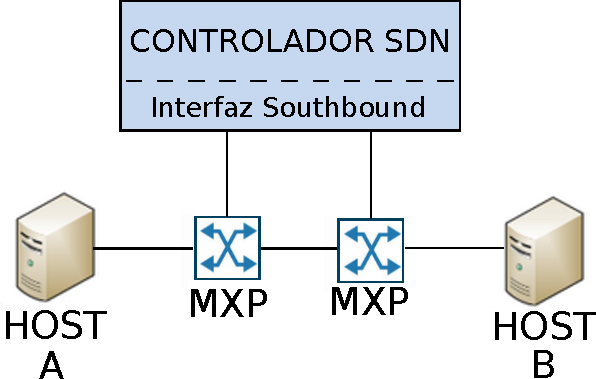
\includegraphics[scale=0.8]{Figures/topologiatest.pdf}
	\caption{Topología utilizada para las pruebas relativas a la integración del protocolo NETCONF.}
	\label{fig:test_topo_netconf}
  \end{figure}


Además, para poder poner a prueba la integración del protocolo con el dispositivo se realizan las siguientes suposiciones y condiciones previas:

\begin{itemize}
	\item El host y el muxponder deben tener conectividad entre sí.
    \item Se debe tener instalado en el host, el cliente yangcli.
    \item Tener instalado en el muxponder, el agente netconfd.
    \item Tanto el módulo YANG como la librería desarrollada para el muxponder, deben estar instalados en el mismo.
    \item La aplicación “monitor” debe estar iniciada en el muxponder.
    \item El equipo no tiene ninguna configuración previa aplicada.
\end{itemize}


\subsection{Casos de prueba y resultados}

A continuación, se proponen una serie de cuadros que presentan la descripción de los procedimientos llevados a cabo para probar los requerimientos de esta pieza de software. Algunos de los casos de pruebas pueden estar acompañados por imágenes para esclarecer su funcionamiento.

\subsubsection{Caso de Prueba T-R-01}
Se pondrá a prueba el inicio de la sesión NETCONF entre el cliente y el servidor. La figura \ref{fig:test1} presenta la descripción, los procedimientos y los resultados del mismo. 


\begin{figure}[H]
	\centering
	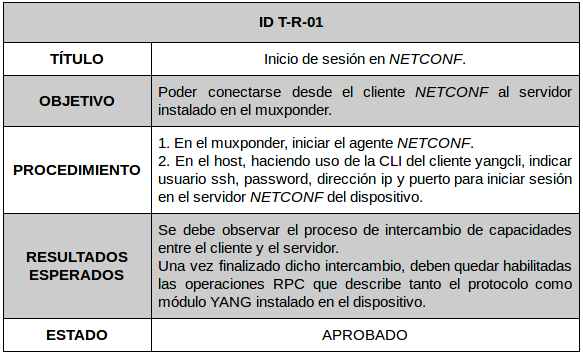
\includegraphics[scale=0.6]{Figures/test_uno.png}
	\caption{Prueba de inicio de sesión.}
	\label{fig:test1}
  \end{figure}



  \subsubsection{Caso de Prueba T-R-02}
  En este caso, se pone a prueba las consultas por los datos de estado y de configuración del módulo YANG. Los procedimientos para esta prueba y sus resultados se presentan en la figura \ref{fig:test2}. 



\begin{figure}[H]
	\centering
	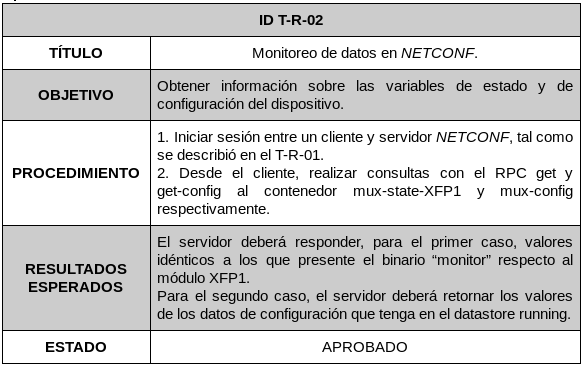
\includegraphics[scale=0.6]{Figures/test2.png}
	\caption{Prueba de monitoreo de datos.}
	\label{fig:test2}
  \end{figure}

  Por otra parte, la figura \ref{fig:test2_consulta} ejemplifica el resultado de una operación de consulta al container mux-state-XFP1, el cual contiene información de estado de dicho módulo XFP.


  \begin{figure}[H]
	\centering
	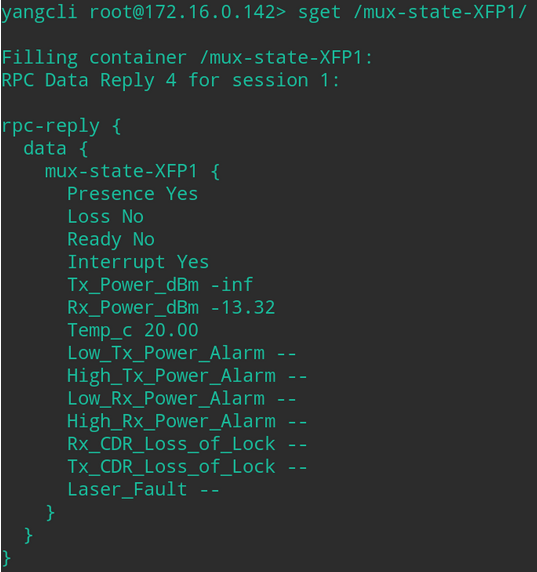
\includegraphics[scale=0.6]{Figures/test2_consulta.png}
	\caption{Monitoreo de datos de estado del container mux-state-XFP1.}
	\label{fig:test2_consulta}
  \end{figure}


  \subsubsection{Caso de Prueba T-R-03}
  Del mismo modo, la figura \ref{fig:test3} detalla los procedimientos que se siguieron para verificar el funcionamiento de la RPC “mux-apply-config” y las notificaciones. Cabe destacar que como se aclaró en las suposiciones para las pruebas, el equipo no se encuentra configurado, por lo que tendrán alarmas referidas a la transmisión y la recepción, entre otras. 


\begin{figure}[H]
	\centering
	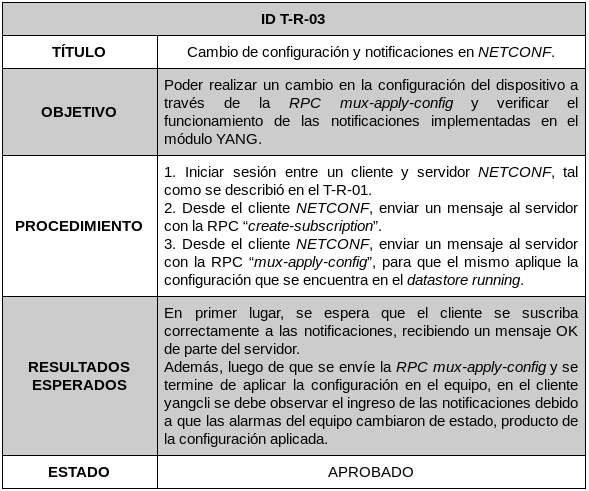
\includegraphics[scale=0.6]{Figures/test3.png}
	\caption{Prueba de cambio de configuración y notificaciones.}
	\label{fig:test3}
  \end{figure}

  La figura \ref{fig:test3_consulta} muestra en primer lugar cómo el cliente se suscribe a las notificaciones mediante la RPC create-suscription. Luego, se puede observar el envío de la RPC mux-apply-config. Seguidamente se muestran las notificaciones entrantes, producto del cambio de estado de las alarmas presentes en el equipo.
  
  \begin{figure}[H]
	\centering
	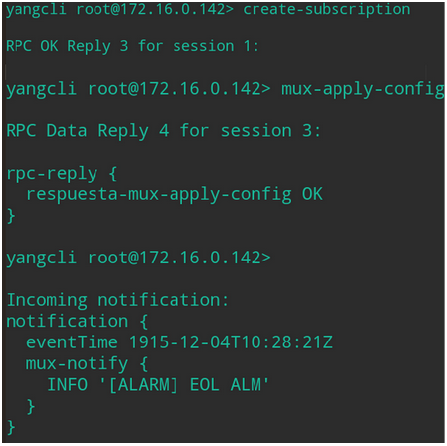
\includegraphics[scale=0.6]{Figures/test3_consulta.png}
	\caption{Suscripción y RPC mux-apply-config.}
	\label{fig:test3_consulta}
  \end{figure}



  %----------------------------------------------------------------------------------------
%	SECTION 2
%----------------------------------------------------------------------------------------

\section{Verificación del driver}

A continuación, en esta sección se pondrá a prueba el driver desarrollado para el controlador ONOS. Los requerimientos los cuales se deben asegurar su cumplimiento son los que se observan en la figura \ref{fig:req_driver}. 


\subsection{Matriz de trazabilidad}

A fines de poner a prueba el cumplimiento de los requerimientos para esta pieza de software, se desarrollan dos casos de prueba. 

En el primero, se verifica que el controlador sea capaz de descubrir correctamente la información de los dispositivos agregados a la topología. 

La segunda prueba abarca la verificación tanto de la función LinkDiscovery como la RPC mux-apply-config. Además, para ambas pruebas se utilizan los comandos CLI implementados en el driver.

De esta forma, resulta la matriz de trazabilidad que se observa en el cuadro \ref{tab:matriz_driver}.


\begin{table}[!h]
    \centering
    \begin{tabular}{|c|c|c|}
        \hline
        \textbf{}     & \textbf{T-R-04} & \textbf{T-R-05} \\ \hline
        \textbf{R-11} & \textit{X}      & \textit{}       \\ \hline
        \textbf{R-12} & \textit{}       & \textit{X}      \\ \hline
        \textbf{R-13} & \textit{}       & \textit{X}      \\ \hline
        \textbf{R-14} & \textit{X}      & \textit{X}      \\ \hline
        \end{tabular}
    \caption{Matriz de trazabilidad - Verificación del driver}
    \label{tab:matriz_driver}
\end{table}

\subsection{Escenario}

En este caso, la topología utilizada para las pruebas es la que se muestra en la figura \ref{fig:test_topo_netconf}. Se tendrán dos muxponders conectados entre sí a través de las interfaces de línea de los mismos. Por otra parte, el controlador ONOS estará conectado a la interfaz de control de ambos dispositivos. 


\begin{figure}[!h]
	\centering
	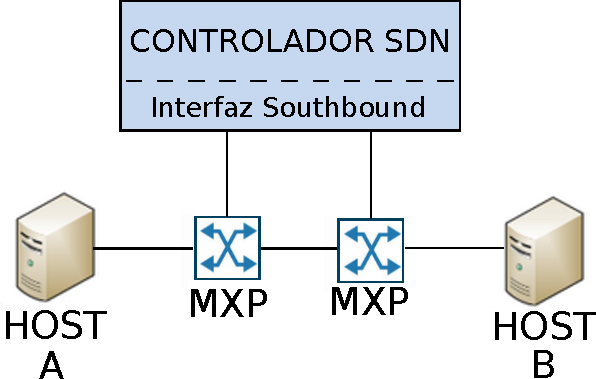
\includegraphics[scale=0.8]{Figures/topologiatest.pdf}
	\caption{Topología utilizada para las pruebas relativas al driver.}
	\label{fig:test_topo_netconf}
  \end{figure}


  Además, se realizan las siguientes suposiciones:

\begin{itemize}
	\item Los agentes netconfd se encuentran iniciados en ambos dispositivos.
    \item Tanto el módulo YANG como la librería en C desarrollada para los muxponders, están instaladas en los mismos.
    \item La aplicación “monitor” está iniciada en ambos muxponders.
    \item Los dispositivos no tienen una configuración previa instalada. 
    \item Los equipos no tienen información relacionada a la presencia de vecinos.
\end{itemize}


\subsection{Casos de prueba y resultados}

\subsubsection{Caso de Prueba T-R-04}

Se pondrá a prueba la función llamada “DeviceDescriptionDiscovery”, la cual como se explicó en el capítulo anterior, es la encargada de registrar en el controlador información adicional de los equipos. Tanto la descripción como los procedimientos llevados a cabo y los resultados de los mismos se presentan en el cuadro [x]. 

\begin{figure}[H]
	\centering
	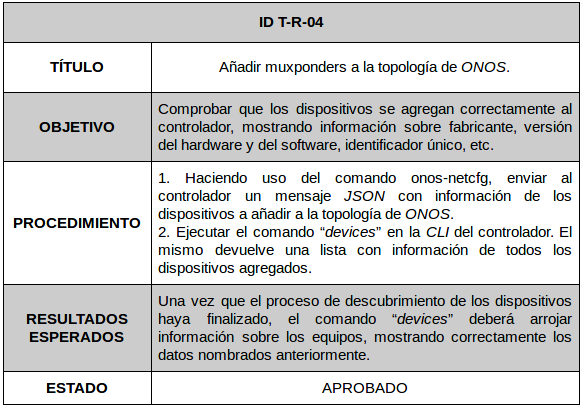
\includegraphics[scale=0.6]{Figures/test4.png}
	\caption{Prueba de DeviceDescriptionDiscovery.}
	\label{fig:test2}
  \end{figure}

  Se observa en la figura \ref{fig:test4_consulta} los dispositivos agregados a la topología de ONOS. Al hacer click sobre cualquier de ellos, el controlador despliega un cuadro del dispositivo seleccionado mostrando la información mencionada anteriormente.

  \begin{figure}[H]
	\centering
	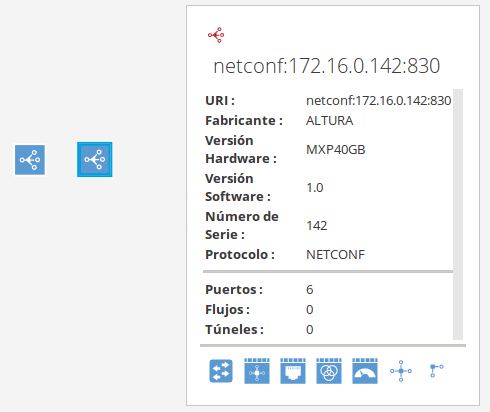
\includegraphics[scale=0.5]{Figures/test4_consulta.png}
	\caption{Dispositivos presentes en la topología de ONOS.}
	\label{fig:test4_consulta}
  \end{figure}


  \subsubsection{Caso de Prueba T-R-05}

  Este caso pone a prueba tanto la función “LinkDiscovery”, la cual es la encargada de formar los enlaces entre los distintos dispositivos, como la RPC mux-apply-config. 
  En el cuadro [x] se detalla la descripción del caso de prueba mencionado. Se asumirá que los dispositivos ya se encuentran añadidos al controlador.
  

\begin{figure}[H]
	\centering
	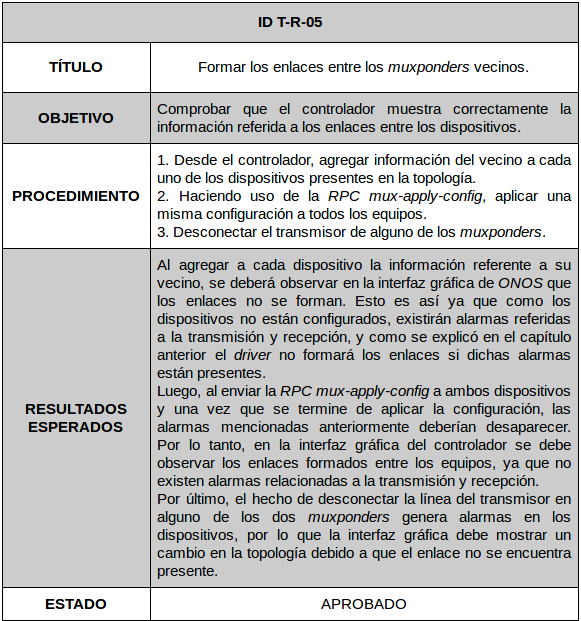
\includegraphics[scale=0.6]{Figures/test5.png}
	\caption{Prueba de LinkDiscovery y mux-apply-config.}
	\label{fig:test5}
  \end{figure}

  La figura X muestra la topología presente en el controlador una vez se le indicó a cada dispositivo la presencia de un vecino. Como se puede notar, el controlador no forma los enlaces entre los mismos ya que los dispositivos contienen alarmas debido a que no están configurados. 

  \begin{figure}[H]
	\centering
	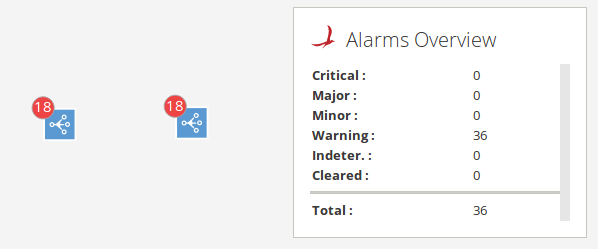
\includegraphics[scale=0.5]{Figures/test5_1.png}
	\caption{Dispositivos presentes en la topología de ONOS.}
	\label{fig:test4_consulta}
  \end{figure}

  A su vez, en la figura x se observa que una vez aplicada la configuración en ambos dispositivos, la cantidad de alarmas presentes se reducen, y al no existir alarmas referidas a la transmisión y recepción de los equipos el controlador puede formar correctamente el enlace entre los mismos. 

  \begin{figure}[H]
	\centering
	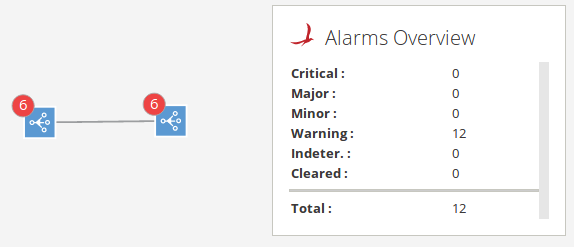
\includegraphics[scale=0.5]{Figures/test5_2.png}
	\caption{Dispositivos presentes en la topología de ONOS.}
	\label{fig:test4_consulta}
  \end{figure}

  Por último, la figura X ejemplifica lo que sucede cuando se desconecta el transmisor en alguno de los dispositivos, provocando la caída de un enlace en la topología de ONOS.

  \begin{figure}[H]
	\centering
	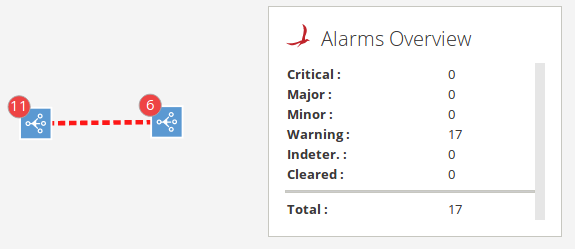
\includegraphics[scale=0.5]{Figures/test5_3.png}
	\caption{Dispositivos presentes en la topología de ONOS.}
	\label{fig:test4_consulta}
  \end{figure}



    %----------------------------------------------------------------------------------------
%	SECTION 3
%----------------------------------------------------------------------------------------

\section{Verificación de la interfaz gráfica y la interfaz REST}

Finalmente, en esta sección se pondrán a prueba ambas interfaces desarrolladas. Para ello, las pruebas realizadas tendrán como objetivo validar el cumplimiento de los requerimientos vistos en la figura [x]. 

Además, los casos de prueba presentados a continuación harán uso tanto del driver como de la aplicación C desarrollada para el agente NETCONF.


\subsection{Matriz de trazabilidad}

Se presenta a continuación en el cuadro [x] la matriz de trazabilidad para las pruebas realizadas. 
En la primer prueba, se verifica poder agregar dispositivos a través de la interfaz gráfica y configurar ambos como vecinos. 
Luego, se verifica en la prueba T-R-07 que puedan visualizarse las alarmas en la aplicación WEB.
Por otra parte, en la prueba T-R-08 se verifica que sea posible visualizar haciendo uso de la interfaz gráfica, cualquier dato de estado de los dispositivos.
Por último se prueba realizar un cambio en la configuración en los dispositivos de tal forma que se permita la conectividad entre los host.



\begin{table}[!h]
    \centering
    \begin{tabular}{|c|c|c|}
        \hline
        \textbf{}     & \textbf{T-R-04} & \textbf{T-R-05} \\ \hline
        \textbf{R-11} & \textit{X}      & \textit{}       \\ \hline
        \textbf{R-12} & \textit{}       & \textit{X}      \\ \hline
        \textbf{R-13} & \textit{}       & \textit{X}      \\ \hline
        \textbf{R-14} & \textit{X}      & \textit{X}      \\ \hline
        \end{tabular}
    \caption{Matriz de trazabilidad - Verificación del driver}
    \label{tab:matriz_driver}
\end{table}

\subsection{Escenario}

La topología utilizada para las pruebas mencionadas anteriormente, es la que se muestra en la figura [x]. 
Se tendrán dos muxponders conectados entre sí a través de las interfaces de línea de los mismos. Además, el controlador ONOS estará conectado a la interfaz de control de ambos dispositivos. Por último, se tienen dos computadoras de propósito general conectadas a los módulos XFP1 de los muxponders.



\begin{figure}[!h]
	\centering
	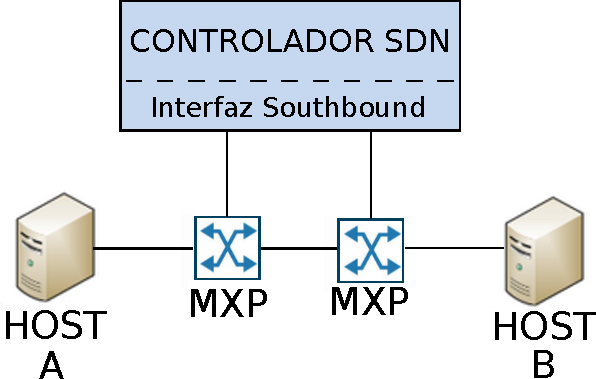
\includegraphics[scale=0.8]{Figures/topologiatest.pdf}
	\caption{Topología utilizada para las pruebas relativas al driver.}
	\label{fig:test_topo_netconf}
  \end{figure}


  Además, se realizan las siguientes suposiciones:

\begin{itemize}
	\item Los agentes netconfd se encuentran iniciados en ambos dispositivos.
    \item Tanto el módulo YANG como la librería en C desarrollada para los muxponders, están instaladas en los mismos.
    \item La aplicación “monitor” está iniciada en ambos muxponders.
    \item Los dispositivos no tienen una configuración previa instalada. 
    \item Los equipos no tienen información relacionada a la presencia de vecinos.
\end{itemize}


\subsection{Casos de prueba y resultados}

\subsubsection{Caso de Prueba T-R-06}

A continuación, se pondrá a prueba agregar nuevos dispositivos a la topología del controlador desde la interfaz gráfica y configurar a los mismos como vecinos. Los procedimientos llevados a cabo para dicha prueba se observan en el cuadro [x].


\begin{figure}[H]
	\centering
	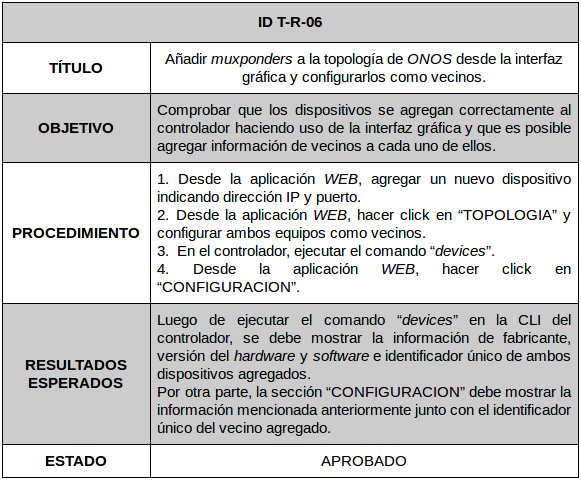
\includegraphics[scale=0.6]{Figures/test6.png}
	\caption{Prueba de DeviceDescriptionDiscovery.}
	\label{fig:test2}
  \end{figure}



  \subsubsection{Caso de Prueba T-R-07}

El objetivo del caso de prueba presentado en el cuadro [x], es el de verificar que la interfaz gráfica presente de forma correcta la información relacionada a las alarmas en los dispositivos. 
Se hará uso tanto de la aplicación “monitor” como de los comandos “alarms” y “alarms-count” de ONOS para validar las alarmas presentes.


\begin{figure}[H]
	\centering
	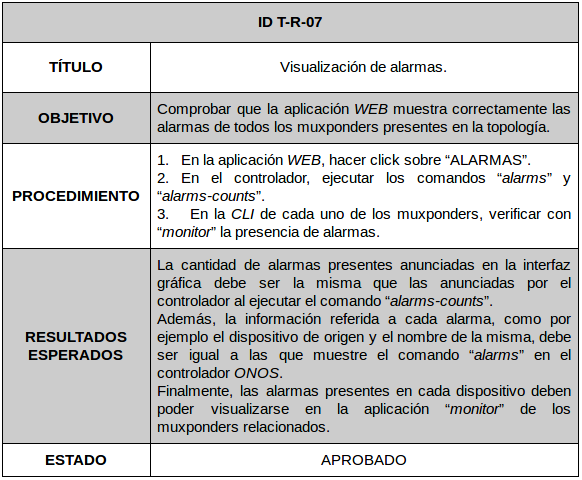
\includegraphics[scale=0.6]{Figures/test7.png}
	\caption{Prueba de DeviceDescriptionDiscovery.}
	\label{fig:test2}
  \end{figure}

  Tal y como se puede ver en la figura [x], se tienen 12 alarmas presentes referidas a los módulos XFP2, XFP3 y XFP4 de ambos dispositivos.

  \begin{figure}[H]
	\centering
	\resizebox{\textwidth}{!}{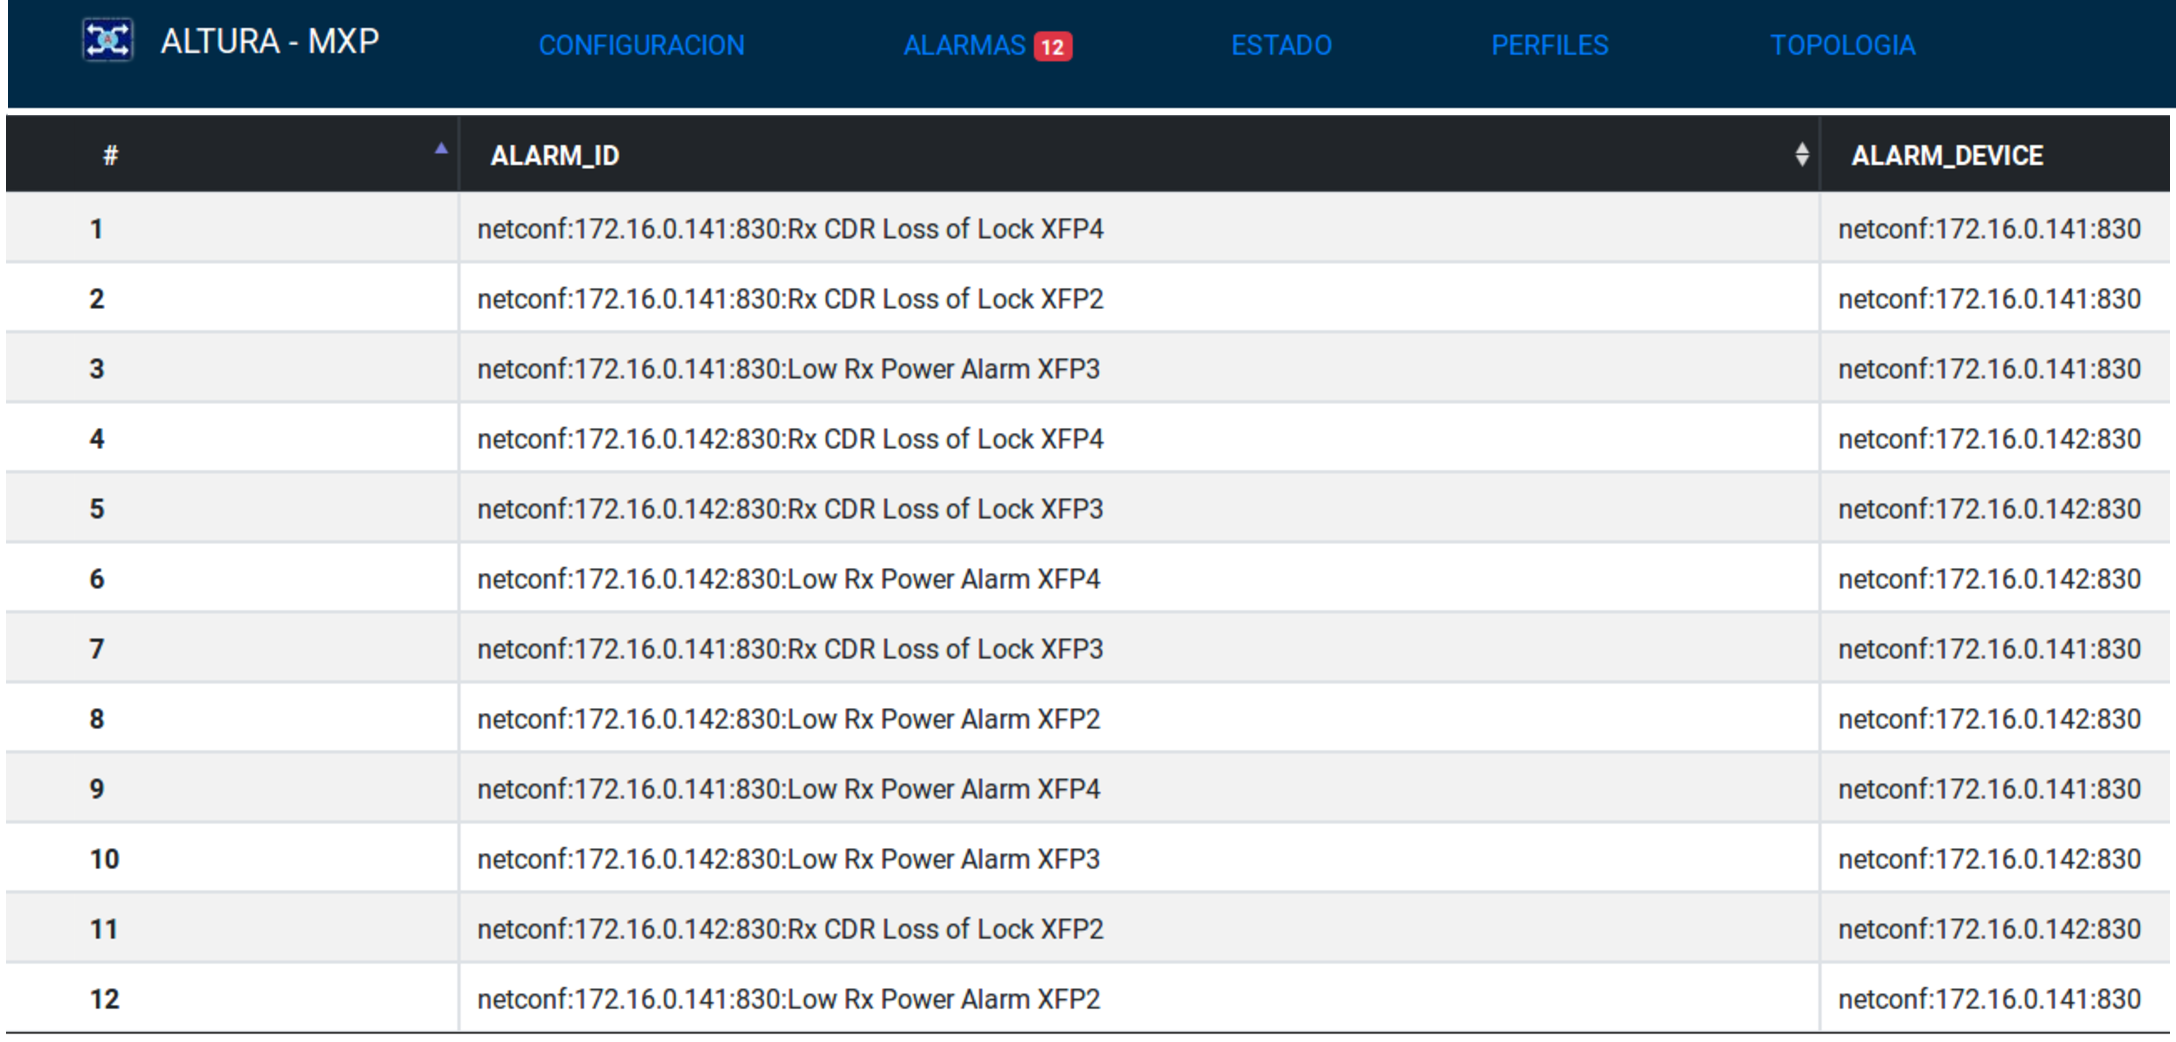
\includegraphics{Figures/test7_1.pdf}}
	\caption{Prueba de DeviceDescriptionDiscovery.}
	\label{fig:test2}
  \end{figure}

  Para comprobar dichas alarmas, se ejecutaron los comandos alarms y alarms-counts los cuales listan las alarmas presentes en el controlador. Se puede ver en la figura [x] la salida del comando alarms-counts, la cual anuncia la misma cantidad de alarmas presentes que lo mostrado por la interfaz.

  \begin{figure}[H]
	\centering
	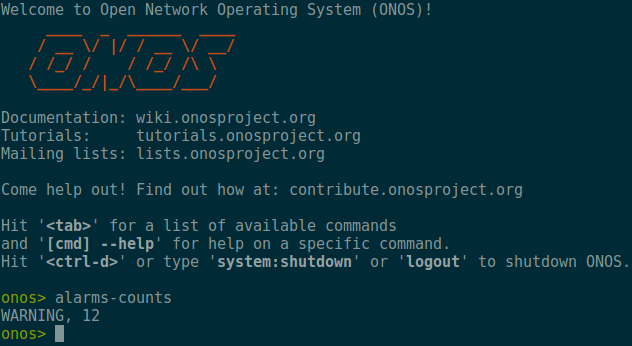
\includegraphics[scale=0.5]{Figures/test7_2.png}
	\caption{Prueba de DeviceDescriptionDiscovery.}
	\label{fig:test2}
  \end{figure}

  Por último, se muestra en la figura [x] la salida del binario “monitor” de uno de los muxponder. En ella, es posible observar 6 etiquetas “Alarm” en la seccion de modulos XFP. Teniendo en cuenta que se tiene el mismo resultado en el otro dispositivo, se tienen las 12 alarmas en total.

  \begin{figure}[H]
	\centering
	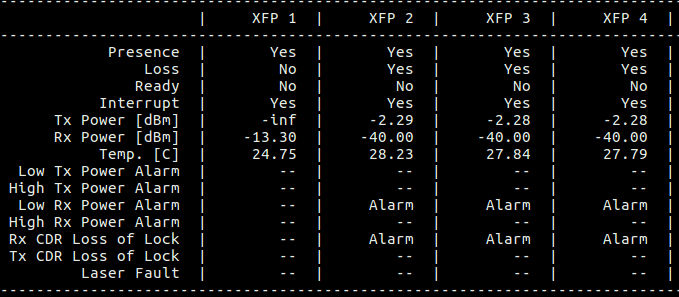
\includegraphics[scale=0.5]{Figures/test7_3.png}
	\caption{Prueba de DeviceDescriptionDiscovery.}
	\label{fig:test2}
  \end{figure}

  \subsubsection{Caso de Prueba T-R-08}

  Se presenta la prueba que se observa en el cuadro [x], la cual tiene como objetivo verificar que es posible observar cualquier dato de estado del dispositivo a través de la interfaz gráfica. Al igual que en la prueba anterior, se hará uso del binario “monitor” para comprobar su funcionamiento.
  
  
  \begin{figure}[H]
      \centering
      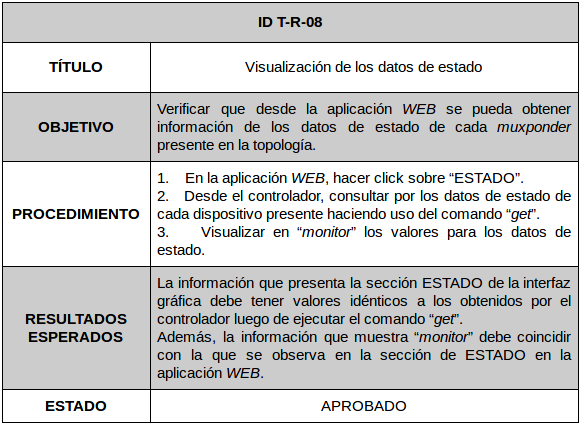
\includegraphics[scale=0.6]{Figures/test8.png}
      \caption{Prueba de DeviceDescriptionDiscovery.}
      \label{fig:test2}
    \end{figure}

    A continuación, en la figura [x] se muestran los valores obtenidos referidos al container “misc” de ambos dispositivos. 

    \begin{figure}[H]
        \centering
        \resizebox{\textwidth}{!}{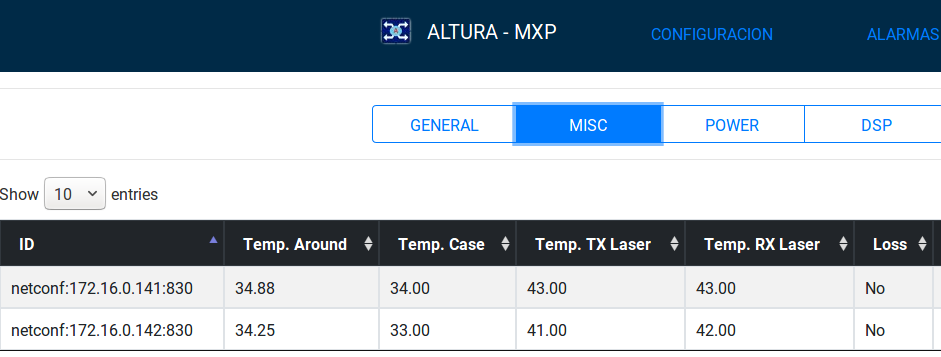
\includegraphics{Figures/test8_1.png}}
        \caption{Prueba de DeviceDescriptionDiscovery.}
        \label{fig:test2}
      \end{figure}

      Por otra parte, se observa en la figura [x] la sección referida a misc en monitor, los cuales tal como se pueden ver tienen los mismos valores que los obtenidos por la interfaz gráfica. 
      
      Es importante aclarar que debido a la cantidad de los datos presentes en este container, las figuras nombradas anteriormente solo muestran una porción de los datos.
      
      Así, se observan únicamente los primeros cinco valores.

      \begin{figure}[H]
        \centering
        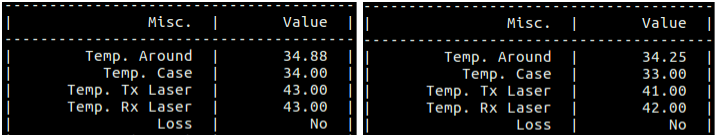
\includegraphics[scale=0.5]{Figures/test8_2.png}
        \caption{Prueba de DeviceDescriptionDiscovery.}
        \label{fig:test2}
      \end{figure}

      \subsubsection{Caso de Prueba T-R-09}

      Por último, el caso de prueba mostrado en el cuadro [x] tiene como objetivo verificar que es posible configurar los muxponders de tal manera que los host A y B tengan conectividad entre sí. 

      \begin{figure}[H]
        \centering
        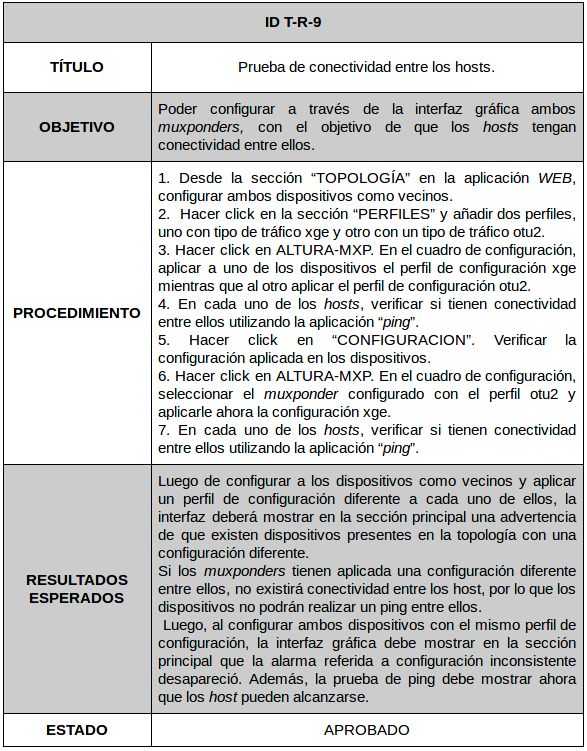
\includegraphics[scale=0.5]{Figures/test9.png}
        \caption{Prueba de DeviceDescriptionDiscovery.}
        \label{fig:test2}
      \end{figure}

      La figura [x] muestra la sección principal de la interfaz gráfica. En ella, es posible observar un recuadro en amarillo indicando que se detectó una configuración inconsistente entre los dispositivos (o sea, que los dispositivos vecinos no tienen la misma configuración). 

      \begin{figure}[H]
        \centering
        \resizebox{\textwidth}{!}{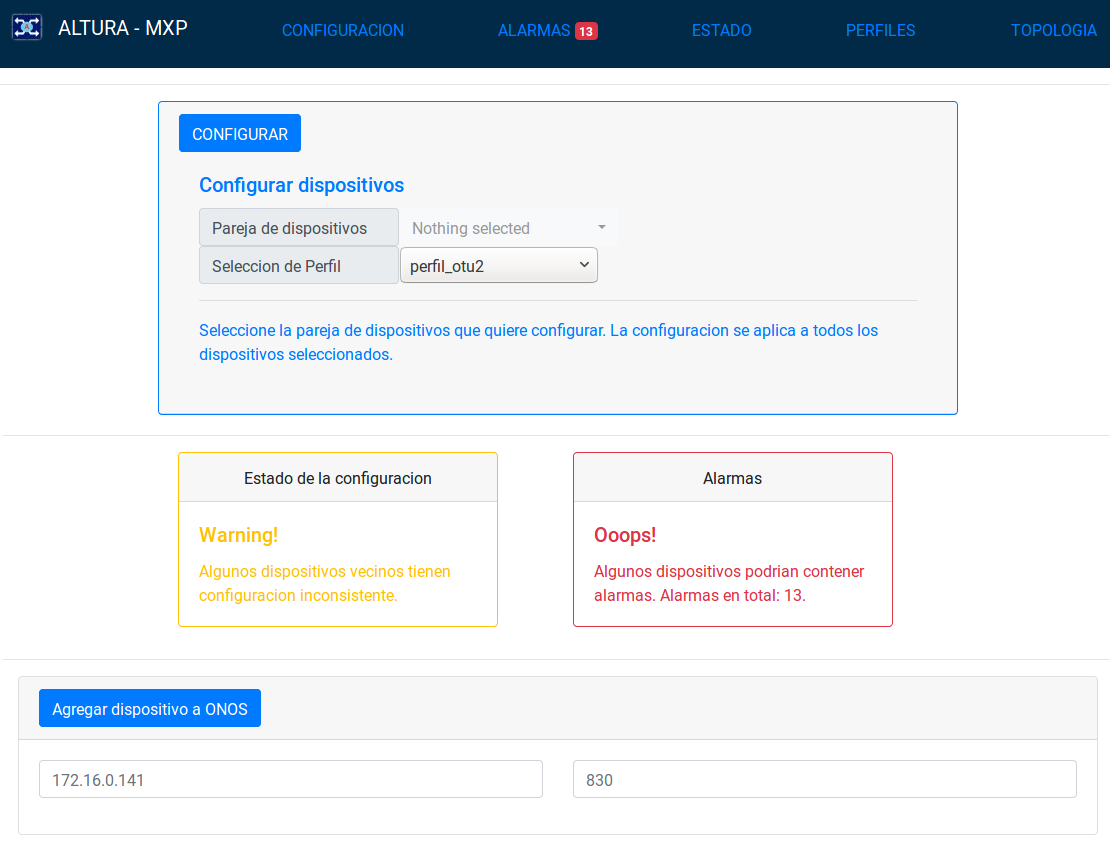
\includegraphics{Figures/test9_1.png}}
        \caption{Prueba de DeviceDescriptionDiscovery.}
        \label{fig:test2}
      \end{figure}

      En este punto, si los host tratan de realizar un ping entre ellos el resultado es el que se puede ver en la figura [x]. Como se esperaba, los hosts no tienen conectividad entre ellos debido a la configuración inconsistente aplicada a los dispositivos.

      \begin{figure}[H]
        \centering
        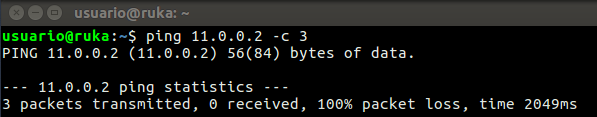
\includegraphics[scale=0.7]{Figures/test9_2.png}
        \caption{Prueba de DeviceDescriptionDiscovery.}
        \label{fig:test2}
      \end{figure}

      Luego, al configurar ambos dispositivos con el perfil de configuración xge, la interfaz muestra que la alarma debido a configuración inconsistente desapareció, tal y como se muestra en la figura x.


      \begin{figure}[H]
        \centering
        \resizebox{\textwidth}{!}{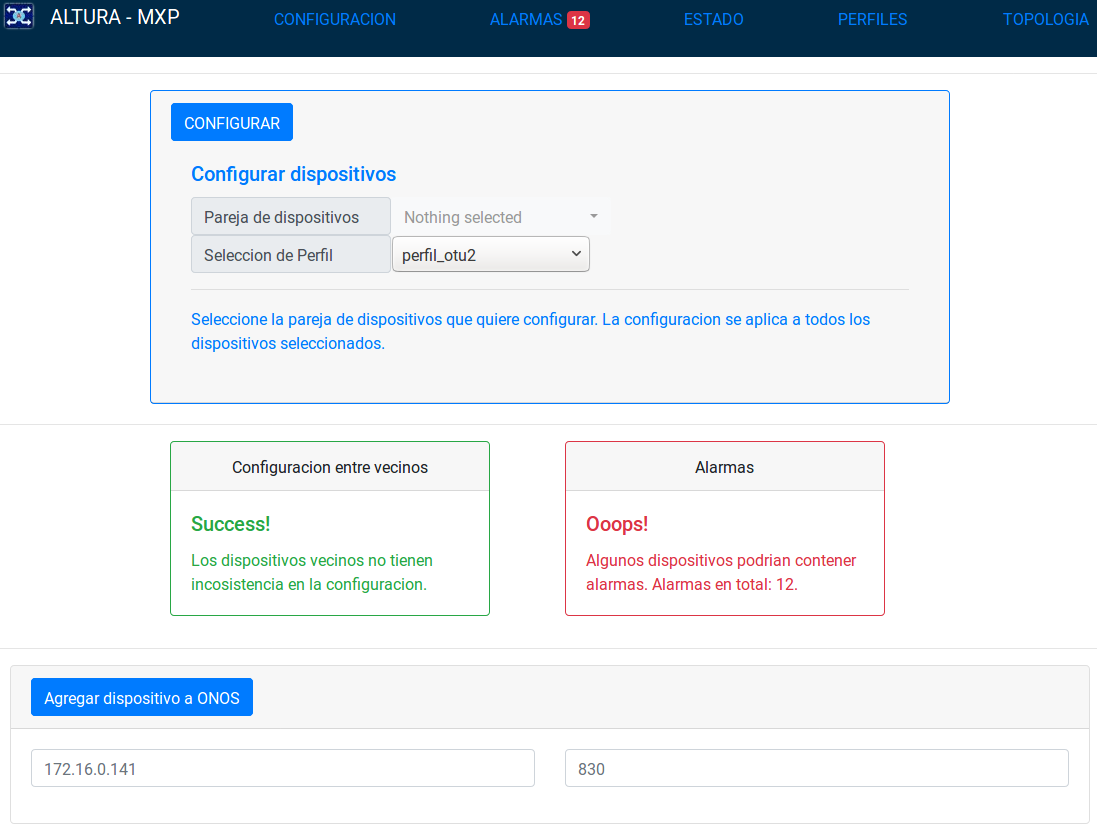
\includegraphics{Figures/test9_3.png}}
        \caption{Prueba de DeviceDescriptionDiscovery.}
        \label{fig:test2}
      \end{figure}

      Por último, se realiza nuevamente la prueba de conectividad realizando un ping entre los hosts. Como se puede ver en la figura [x], los clientes ahora tienen conectividad entre ellos.

      \begin{figure}[H]
        \centering
        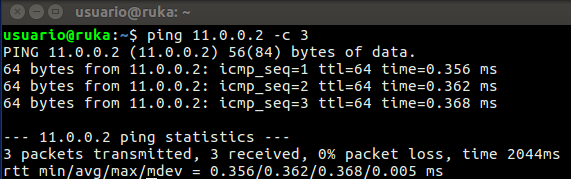
\includegraphics[scale=0.7]{Figures/test9_4.png}
        \caption{Prueba de DeviceDescriptionDiscovery.}
        \label{fig:test2}
      \end{figure}
